\documentclass[12pt,letterpaper]{report}
\usepackage{natbib, url, tablefootnote, tipa}
\usepackage{geometry}
\usepackage{fancyhdr}
\usepackage{afterpage}
\usepackage{graphicx, caption, epstopdf, multirow}
\usepackage{amsmath,amssymb,amsbsy}
\usepackage{dcolumn,array}
\usepackage{tocloft}
\usepackage{asudis}
\usepackage[pageanchor=true,plainpages=false,pdfpagelabels,bookmarks,bookmarksnumbered]{hyperref}

\begin{document}
%-----------------------front matter
\pagenumbering{roman}
\title{A computational model for studying L1's effect on L2 learning}
\author{Ming Tu}
\degreeName{Doctor of Philosophy}
\paperType{Dissertation}
\defensemonth{August}
\defenseyear{2018}
\gradmonth{August}
\gradyear{2018}
\memberOne{Dr. Visar Berisha}
\memberTwo{Dr. Julie Liss}
\memberThree{Dr. Yi Zhou}

\maketitle
\doublespace
\begin{abstract}
Much evidence has shown that first language (L1) plays an important role in the formation of L2 phonological system during second language (L2) learning process. This combines with the fact that different L1s have distinct phonological patterns to indicate the diverse L2 learning outcomes for speakers from different L1 backgrounds. Usually, accented speech is investigated with either segmental (short-term speech measurements on short-segment or phoneme level) or suprasegmental (long-term speech measurements on word, long-segment, or sentence level) measurements. This dissertation hypothesizes that phonological distances between accented speech and speakers' L1 are negatively correlated with perceived accentedness. Moreover, contrastive phonological distinctions between L1s and L2 will manifest themselves in the accented speech produced by speaker from these L1s.

To test the hypotheses, this study comes up with a computational model to analyze the accented speech properties in both segmental and suprasegmental feature space. The core parts of this computational model are feature extraction schemes to extract pronunciation and prosody representation of accented speech based on existing techniques in automatic speech recognition field. Correlation analysis on both segmental and suprasegmental feature space is conducted to look into the L1's influence on accentedness perception across several L1s. Multiple regression analysis is employed to investigate how the L1's effect impacts the perception of foreign accent perception, and how accented speech produced by speakers from different L1s behaves distinctly on segmental and suprasegmental feature spaces. Results unveil the potential application of the methodology in this study to provide quantitative analysis of accented speech and extend current studies in L2 learning theory to large scale. Practically, this study further shows that the computational model proposed in this study can benefit automatic accentedness evaluation system by adding features related to speakers' L1s.
\end{abstract}

\dedicationpage{To my parents, my wife and my lovely daughter}
\include{ack}
\tableofcontents
% This puts the word "Page" right justified above everything else.
\addtocontents{toc}{~\hfill Page\par}
% Asking LaTeX for a new page here guarantees that the LOF is on a separate page
% after the TOC ends.
\newpage
% Making the LOT and LOF "parts" rather than chapters gets them indented at
% level -1 according to the chart: top of page 4 of the document at
% ftp://tug.ctan.org/pub/tex-archive/macros/latex/contrib/tocloft/tocloft.pdf
\addcontentsline{toc}{part}{LIST OF TABLES}
\renewcommand{\cftlabel}{Table}
\listoftables
% This gets the headers for the LOT right on the first page.  Subsequent pages
% are handled by the fancyhdr code in the asudis.sty file.
\addtocontents{lot}{Table~\hfill Page \par}
\newpage
\addcontentsline{toc}{part}{LIST OF FIGURES}
\addtocontents{toc}{CHAPTER \par}
\renewcommand{\cftlabel}{Figure}
% This gets the headers for the LOF right on the first page.  Subsequent pages
% are handled by the fancyhdr code in the asudis.sty file.
\addtocontents{lof}{Figure~\hfill Page \par}
\listoffigures
%-----------------------body
\doublespace
\pagenumbering{arabic}
\chapter{Introduction}
\label{introduction}

\section{Problem Statement}
Languages are different. Linguistic typology studies classification of world languages depending their structural and functional features. Because of the diversity of different languages, there are many criterion defined to classify languages into different groups \citep{wals}. For example, according to subject-verb-object positioning, languages can be grouped into different sets: SOV (such as French, German, Spanish and Chinese), SVO (such as English and Chinese) and so on, where the abbreviation represents the order of subject(S), verb(V) and object(O). Phonologically, patterns in the structure and distributions of sound systems are investigated to classify world's languages based on phonological properties. As summarized by \citep{wals}, properties including vowel and consonant inventory, consonant-vowel ratio, syllable structure, rhythm types, etc. are used to represent the difference in phonology across different languages. Some of those properties mainly measure segmental information while others measure supra-segmental information of one language's phonological system. Those various phonological properties result in diverse acoustic characteristics when we listen to speech recordings in different languages. Another important outcome of the those different phonological properties across languages is that when a speaker speaks in a language other than his mother tongue the speech he will be perceived to have accent, which comes from the interplay of the phonological difference of the first language (L1, the speaker's mother tongue) and second language(L2, the language the speaker is speaking). Accented speech is the focus of the study in this dissertation.

Accented speech is the result of L2 speech being produced by a sensorimotor control system that has overlearned L1 phonological patterns, including both phoneme sound contrasts and rhythmic composition. According to L1 acquisition theory, the malleability of human brain in terms of language is strongest only for a limited time (sometime between age 5 and puberty), which is referred as the critical period hypothesis. After that period, language acquisition is much more difficult. The critical period hypothesis from L1 acquisition was extended to include L2 acquisition, positing that a critical age or period after which L2 speech production could not be native like \citep{long1990maturational}. However, further research revealed that the speech learning model (SLM) accounted for exceptions that can not be explained by the critical period hypothesis. For example, it was reported that both early L2 learners failed to achieve native-like production while late L2 learners did \citep{flege1995second}. The SLM also hypothesized a shared phonological space for speech sounds and used ``equivalence classification'' to explain why a learner might not create a new phonetic category for an L2 sound perceived as similar to an L1 sound. In addition, findings in neuroscience favored the concept of a ``sensitive'' or ``optimal'' period over a ``critical'' one.

Accentedness is usually used to measure the perceived difference between accented speech produced by L2 learners and speech produced by native speakers. There are multiple ways to define accentedness. A more general definition in literature was proposed in \citep{mccullough2013acoustic} considering previous definitions: accentedness refers to perception of deviations from a pronunciation norm that a listener attributes to the talker not speaking the target language natively. This definition focuses on the difference of the pronunciation of foreign accented speech compared to speech produced by native speakers. In second language learning and education practice, accentedness evaluation is very important to designing specific learning targets for different learners based on their level of accentedness, monitoring the learning progress and qualifying or quantifying the learning outcomes. One common experimental design in the study of perceived foreign accent is to have participants rate the degree of accentedness in various auditory stimuli, and then to relate these ratings to properties measured in the stimuli. Much research has been done to study the relationship between perceived foreign accent and acoustic characteristics of accented speech, such as voice onset time (VOT) \citep{major1987english}, word duration, stressed or unstressed vowel duration ratio \citep{shah2002temporal}, formants movement deviation from L1 acoustic values \citep{munro1993productions}, etc. In addition to the largely segmental acoustic properties suggested by the findings of previous studies, there are also some works focusing on supra-segmental information, including prosodic and global temporal properties, of foreign accented speech \citep{munro2010detection,kang2010relative}. Both those segmental and supra-segmental acoustic measurements have been shown to be correlated with perceived accentedness.

Though it is clear that the perception of accentedness is highly correlated with how far the phonological patterns of produced accented speech is from patterns of native speech, what has not been studied is whether the distance to the phonological patterns of the speaker's mother tongue matters. According to SLM, phonetic systems of L2 learners responds to L2 sounds by adding new phonetic categories, or modifying existing L1 phonetic categories \citep{flege1995second}. SLM claims that a new phonetic categories may be formed for an L2 sound given sufficient dissimilarity from the closest L1 sound and equivalence classification may block the category formation for an L2 sound, thus the original L1 phonetic category will be used to process both L1 and L3 sound, resulting in similar L2 production with L1 sound. Since SLM mainly focuses on the phonetic system, following studies also investigate the acquisition of L2 rhythm patterns \citep{rasier2007prosodic,ordin2015acquisition}. The findings in these studies reveal that while the general trend is becoming closer to the L2 rhythm patterns as the accent is milder, there still exist effects of L1 rhythm patterns for speakers from different L1 groups. Based those observation, we may ask

\begin{enumerate}
\item how the distance from the functional phonological system for accented speech to the actual L1 phonological system correlates with the perceived accentedness? Is the position of the phonological patterns of accented speech in the L1 and L2 phonological space a better choice to model the perception of accentedness?
\item Different L1s are at different relative positions with L2 in subspaces of the phonological system, mainly phonetic space and rhythmic space. For example, German and English are both stress-timed languages and thus are closer to each other on rhythmic space compared to French; Mandarin is syllable-timed language and has very different phonetic inventory compared to English so it is far from English on both subspaces. Will these contrastive properties be transferred to the accented speech during L2 acquisition? Furthermore, will those measurements on rhythmic space contribute more to the perception of accentedness compared to measurements on phonetic space for German speakers speaking English?
\end{enumerate}

The above are the research questions that will be investigated in this dissertation. Specifically, the current study will explore the relationship between measurements of phonological system with perceived accentedness by a computational model that extracts representative features of both phonetic and rhythmic subspaces. Given that the deviation of accented speech from the target L2 phonological patterns highly correlated with the accentedness score, this study investigates whether the deviation of accented speech from the original L1 phonological patterns has negative correlation with the accentedness score (i.e. the higher the deviation is, the milder the accent is); whether integrating measurements related to L1 can improve the modeling capability of accentedness perception; whether contrastive patterns of L1s and target L2 can be transferred to L1 accented speech.

\section{Significance of The Study}

There is a huge population of second (or higher order) language learners nowadays. The number of people living in a second language environment are also increasing with the economic globalization. Good understanding of the process of second language learning and accented speech perception is of great importance to successful speech communication in terms of both education, social science and communication science. The current study investigates the perception of accented speech. It aims to achieve better understanding of how the L1 of speakers with accent affects the perception of accentedness phonologically and how the phonetic system and rhythmic patterns contribute to the perception respectively. With a interdisciplinary research methods combining speech learning and perception theories with speech and language technologies, the current study will influence both the theoretic development of second language learning and accented speech perception and the technologies of Computer Assisted Pronunciation Training (CAPT) and Computer Aided Language Learning (CALL).

\section{Outline of The Dissertation}

The dissertation is divided into 8 chapters. Chapter 2 introduces the general background of the current study by reviewing several bodies of research on second language learning and accent speech perception theories and practices: including differential analysis of world languages, second language learning theories, acoustic characteristics of accented speech and computational model of accentedness perception. The motivation and predictions are then presented based on the literature review. Chapter 3 describes the methodology employed in this study including data collection, acoustic analysis and experimental design. Chapter 4 investigates the influence of L1's phonetic system on the accented speech perception. Chapter 5 investigates the influence of L1's rhythm patterns on the accented speech perception. Chapter 5 combines information of L1's phonetic and rhythmic patterns to build a computational model for better accentedness perception. Chapter 7 provides a general discussion of the experimental results and tries to extend the current theories on second langauge learning and accented speech perception. It also introduced the possible implications to both theoretic and practical studies on accented speech. Chapter 8 concludes the current study.




\chapter{General Background}
\label{literature}

\section{Differential Analysis of Languages}

Language is a system that consists of the development, acquisition, maintenance and use of complex systems of communication, particularly the human ability to do so; and a language is any specific example of such a system. Estimates of the number of human languages in the world vary between 5,000 and 7,000. Languages as communication tools are different in many ways. Recall that when you first learn a second language (L2), the alphabet or words in that language looks so strange, especially for those languages using different sets of characters (for example Chinese and English). You may regard those words as a sequence of graphs without any meanings. Also, when you first listen to a sentence in the L2 or two people talking in L2, the sound waves are just noise to you. However, you are still aware that those sentences either in text or sound format are conveying specific information in a different way from your own language. How languages are different and where do those differences come from?

Language (or linguistic) typology is the science that studies ``similarities and differences among languages that do not stem from shared genetic relationship, language contact, or shared environmental conditions'' \citep{moravcsik_2012}. The goal of language typology is to describe and explain the common properties and structural diversity of the world's languages and how those properties generalize in cross-linguistic case \citep{bickel2001typology}. This discipline includes several subfields, depending on the ways languages are grouped into same class. An introductory categorization is provided in \citep{moravcsik2012introducing}:

\begin{enumerate}
\item Lexical typology: deals with characteristic ways in which language packages semantic material into words. For example, English uses different words for ``foot''/``leg'' and ``finger''/``toe'' while languages like Japanese and Russian use one word to represent ``foot''/``leg'' (``ashi'' in Japanese and ``noga'' in Russian) and ``finger''/``toe'' (``yubi'' in Japanese and ``palec'' in Russian).
\item Syntactic typology: deals with characteristic ways in which language packages words into sentences syntactically. For example, according to subject-verb-object positioning, languages can be grouped into different sets: SOV (such as French, German, Spanish and Chinese), SVO (such as English and Chinese) and so on, where the abbreviation represents the order of subject(S), verb(V) and object(O).
\item Morphological typology: deals with characteristics ways in which language forms words by combining morphemes. For example, morphological typology categorize languages into analytic languages and synthetic languages. Analytic languages, including Chinese and Vietnamese, contain very little inflection (inflection refers to ``the modification of a word to express different grammatical categories such as tense, case, voice, aspect, person, number, gender, and mood''), instead relying on features like word order and auxiliary words to convey meaning while synthetic languages, including most Indo-European languages, form words by affixing a given number of dependent morphemes to a root morpheme and word order is less important for synthetic languages.
\item Phonological typology: dealing with characteristics ways in which sounds are distributed across languages and phonological phenomena such as phoneme inventories, syllable structure, phonological alternations, stree/tone/intonation, prosodic morphology and so on. For example, in terms of consonant-vowel ratio, English has relatively is low and Russian is relatively high. In terms of syllable structure, English is relatively complex while Mandarin is relatively simple \citep{wals}.
\end{enumerate}

As introduced in Chapter \ref{introduction}, the current study focuses on phonological patterns of L1 and L2 and how they affect the phonological patterns of accented speech. The phonological difference among different languages will be introduced in this section. There are several data sources for language typology: UCLA Phonological Segment Inventory Database \citep{maddieson1992ucla}, Word Atlas of Language Structures (WALS) \citep{wals}, URIEL Typological Database \citep{littel2016uriel}, PHOIBLE \citep{phoible}, to name a few. Different databases have different data sources and language samples. Here, the features provided by WALS is used to illustrate the phonological difference among several languages for the reason that WALS provides simple ways to visualize and download the data. Those languages will be the target L1s in later sections of this dissertation.

\begin{figure}[h]
\centering
\captionsetup{justification=centering}
\includegraphics[width = 0.8\linewidth]{figures/WALS_example.pdf}
\caption{Consonant-vowel ratio across sampled languages by WALS. Different colors represent different level of consonant-vowel ratio: blue for low level, light blue for moderately low level, white for average level, magenta for moderately high level and red for high level.}
\label{fig:wals_example}
\end{figure}

First, in figure \ref{fig:wals_example}, the consonant-vowel ratio is used as an example of how phonological patterns are different across world's languages. Higher ratio means there are more consonants and less vowels in that language while lower ratio means the opposite. Take some commonly used languages as examples: English, German and French all have low ratio; Spanish, Persian and Mandarin have average ratio; Russian has high ratio.

\begin{table}[]
\centering
\caption{19 language phonological features summarized by WALS. The last column indicates whether the feature is phonetic or rhythmic feature. For detailed description of each feature, refer to \citep{wals}}
\label{table: wals_feature}
\begin{tabular}{|c|c|}
\hline
Feature name & Phonetic or Rhythmic \\ \hline
Consonant Inventories & Phonetic \\ \hline
Vowel Quality Inventories & Phonetic \\ \hline
Consonant-Vowel Ratio & Rhythmic\tablefootnote{Although Consonant-Vowel Ratio looks like a phonetic feature because it is the ratio of the number of consonants and vowels, most studies regard it as a rhythmic feature \citep{gil1986prosodic}.} \\ \hline
Voicing in Plosives and Fricatives & Phonetic \\ \hline
Voicing and Gaps in Plosive Systems & Phonetic \\ \hline
Uvular Consonants & Phonetic \\ \hline
Glottalized Consonants & Phonetic \\ \hline
Lateral Consonants & Phonetic \\ \hline
The Velar Nasal & Phonetic \\ \hline
Vowel Nasalization & Phonetic \\ \hline
Front Rounded Vowels & Phonetic \\ \hline
Syllable Structure & Rhythmic \\ \hline
Tone & Rhythmic \\ \hline
Fixed Stress Locations & Rhythmic \\ \hline
Weight-Sensitive Stress & Rhythmic \\ \hline
Weight Factors in Weight-Sensitive Stress System & Rhythmic \\ \hline
Rhythm Types & Rhythmic \\ \hline
Absence of Common Consonants & Phonetic \\ \hline
Presence of Uncommon Consonants & Phonetic \\ \hline
\end{tabular}
\end{table}

Next, it is clearer to do differential analysis of different languages with phonological patterns and to illustrate the distance among different languages on phonological feature space. To achieve this, several phonological features pre-summarized by WALS are selected. Based on whether there definitions are segmental or supra-segmental, those features are categorized into phonetic features and rhythmic features. Two groups of features represent language phonological patterns on phonetic space and rhythm space respectively. Table \ref{table: wals_feature} includes those features' names and indicates whether each feature is phonetic or rhythmic\footnote{Downloadable from \url{https://cdstar.shh.mpg.de/bitstreams/EAEA0-7269-77E5-3E10-0/wals_language.csv.zip}}. WALS assigns feature values to languages based on the structural properties of languages that describe one aspect of cross-linguistic diversity. For example, the feature ``Rhythm Types'' has five values: Trochaic (left-hand syllable in the foot is strong), Iambic (right-hand syllable in the foot is strong), Dual (system has both trochaic and iambic feet), Undetermined (no clear foot type) and Absent (no rhythmic stress). Those feature values are stored as a number, usually starting from 1, to represent each categories they belong to. To visualize those languages on a 2-dimensional space, the numeric values of each feature are used. If one feature is not applicable to a language, 0 is used instead. As a result, each language will have a 19-dimensional feature vector representing values of those features in table \ref{table: wals_feature}. Each feature vector is also split into phonetic and rhythmic feature vectors. Since each feature actually indicate a category, to make sure the distances among different categories are the same, one-hot encoding is used to convert the integer feature value to a vector consisting of 0s and 1s. The length of the encoded vector is equal to the number of categories that feature can be. For example, the ``Rhythm Types'' feature has 5 categories. Then, a number of 3 will be encoded as ``00010''. Multidimensional scaling (MDS), which seeks a low-dimensional representation of those feature vectors in which the distances respect well the distances in the original high-dimensional space, is employed to illustrate the 2-dimensional representation of each language in all phonological feature space (as shown in figure \ref{fig:all_mds}), phonetic feature only space (as shown in figure \ref{fig:phonetic_mds}) and rhythmic feature only space (as shown in \ref{fig:rhythmic_mds}) with the encoded language features.

\begin{figure}[!htb]
\centering
\minipage{0.55\textwidth}
  \includegraphics[width=\linewidth]{figures/all_MDS.eps}
  \caption{2D visualization of all features with MDS.}\label{fig:all_mds}
\endminipage\hfill
\\
\minipage{0.55\textwidth}
  \includegraphics[width=\linewidth]{figures/phono_MDS_wals.eps}
  \caption{2D visualization of phonetic only features with MDS.}\label{fig:phonetic_mds}
\endminipage\hfill
\\
\minipage{0.55\textwidth}%
  \includegraphics[width=\linewidth]{figures/rhythmic_MDS.eps}
  \caption{2D visualization of rhythmic only features with MDS.}\label{fig:rhythmic_mds}
\endminipage
\end{figure}

Along with the 2-dimensional visualization, normalized pair-wise distance matrices are also shown in table \ref{table:conf_all} for all features, table \ref{table:conf_phonetic} for phonetic features and table \ref{table:conf_rhythmic} fir rhythmic features. The pairwise distance between two languages is calculated as follows: count the number of different values for corresponding dimensions of the feature vectors of two languages without one-hot encoding. This will result in a $N \times N$ matrix where N is the number of languages; normalize the matrix by the maximum value in the matrix. From the feature visualization and normalized pair-wise distance matrices, it can be found that English, German and French are relatively close to each other on all three feature space while other languages are relative far from those three languages. If English is regarded as L2, German is closest to English on all features space. Furthermore, German is closer to English on rhythmic space than phonetic space. So is French. However, Mandarin and Spanish are closer to English on phonetic space than rhythmic space. One important question this study wants to investigate is that whether those L1 to L2 distance patterns will manifest in the accented speech perception: how the relative importance of segmental features and supra-segmental features relates to the distance to L2 on phonetic and rhythmic space.

\begin{table}[!htb]
\centering
\caption{Normalized pairwise distance on all features space.}
\label{table:conf_all}
\resizebox{0.55\columnwidth}{!}{%
\begin{tabular}{|c|c|c|c|c|c|c|c|}
\hline
 & German & Spanish & French & Russian & Hindi & English & Mandarin \\ \hline
German & 0 & 0.92 & 0.33 & 0.67 & 0.67 & 0.33 & 0.83 \\ \hline
Spanish &  & 0 & 0.83 & 0.67 & 0.75 & 0.67 & 0.50 \\ \hline
French &  &  & 0 & 0.67 & 0.58 & 0.58 & 1.00 \\ \hline
Russian &  &  &  & 0 & 0.42 & 0.58 & 0.75 \\ \hline
Hindi &  &  &  &  & 0 & 0.50 & 0.92 \\ \hline
English &  &  &  &  &  & 0 & 0.83 \\ \hline
Mandarin &  &  &  &  &  &  & 0 \\ \hline
\end{tabular}}
\end{table}

\begin{table}[!htb]
\centering
\caption{Normalized pairwise distance on rhythmic features only space.}
\label{table:conf_phonetic}
\resizebox{0.55\columnwidth}{!}{%
\begin{tabular}{|c|c|c|c|c|c|c|c|}
\hline
 & German & Spanish & French & Russian & Hindi & English & Mandarin \\ \hline
German & 0 & 1.00 & 0.29 & 0.71 & 0.86 & 0.43 & 0.71 \\ \hline
Spanish &  & 0 & 1.00 & 0.57 & 0.71 & 0.57 & 0.43 \\ \hline
French &  &  & 0 & 0.71 & 0.57 & 0.71 & 1.00 \\ \hline
Russian &  &  &  & 0 & 0.29 & 0.57 & 0.71 \\ \hline
Hindi &  &  &  &  & 0 & 0.71 & 0.86 \\ \hline
English &  &  &  &  &  & 0 & 0.71 \\ \hline
Mandarin &  &  &  &  &  &  & 0 \\ \hline
\end{tabular}}
\end{table}

\begin{table}[!htb]
\centering
\caption{Normalized pairwise distance on rhythmic features only space.}
\label{table:conf_rhythmic}
\resizebox{0.55\columnwidth}{!}{%
\begin{tabular}{|c|c|c|c|c|c|c|c|}
\hline
 & German & Spanish & French & Russian & Hindi & English & Mandarin \\ \hline
German & 0 & 0.80 & 0.40 & 0.60 & 0.40 & 0.20 & 1.00 \\ \hline
Spanish &  & 0 & 0.60 & 0.80 & 0.80 & 0.80 & 0.60 \\ \hline
French &  &  & 0 & 0.60 & 0.60 & 0.40 & 1.00 \\ \hline
Russian &  &  &  & 0 & 0.60 & 0.60 & 0.80 \\ \hline
Hindi &  &  &  &  & 0 & 0.20 & 1.00 \\ \hline
English &  &  &  &  &  & 0 & 1.00 \\ \hline
Mandarin &  &  &  &  &  &  & 0 \\ \hline
\end{tabular}}
\end{table}

The previous features are summarized by linguistics on a high systematic level. How those features manifest themselves in the acoustic recordings of different languages? How the languages' differences manifest themselves in the key parameters of acoustic speech signal including intensity, pitch, formants, envelop and so on? Several studies have investigate this and those findings. An early study \citep{parmenter1933experimental} compared the acoustic characteristics between English and French reading speech and showed that pitch is more important as an element of accent than intensity for French speech while intensity is more important for English speech. Also, French speech has more pitch variation than English. Studies in \citep{jongman1989acoustic,bradlow1995comparative,al2005does} investigated the relationship between vowel inventories and vowel space (defined as the two-dimensional area bounded by lines connecting first and second formant frequency coordinates of vowels) and concluded that vowel space depends on the size of vowel inventory: the larger the inventory, the bigger the acoustic space. The work by \citep{wagner2003voice} showed that predominant factors in voice quality are different across different languages. In terms of speech rhythm, an influential study in \citep{ramus1999correlates} studied the representation of linguistic speech rhythm in acoustic speech signal. Several acoustic measurements for speech rhythm are proposed to discriminate the rhythm classes of different languages. Those measurements include the percentage of vocalic segment in an utterance ($\%V$), the standard deviation of consonant intervals ($\Delta C$) and the standard deviation of vowel intervals ($\Delta V$). Figure is taken from \citep{ramus1999correlates} to show how $\%V$ and $\Delta C$ can discriminate languages. Based this study, other measurements like variational coefficient of consonant/vowel intervals \citep{dellwo2006rhythm}, pairwise variability index of consonant/vowel intervals \citep{grabe2002durational} are also proposed. Those studies that correlate those linguistically summarized phonological language features with acoustic measurements lay the foundation of the methodology used in this study.

\begin{figure}[h]
\centering
\captionsetup{justification=centering}
\includegraphics[width = 0.8\linewidth]{figures/ramus_paper.JPG}
\caption{Distribution of languages over the ($\%V$, $\Delta C$) plane. EN: English, PO: Polish, DU: Dutch, SP: Spanish, IT: Italian, FR: French, CA: Catalan, JA: Japanese.}
\label{fig:wals_example}
\end{figure}

\chapter{Methodology Overview}
\label{sec:methodology}
\section{Introduction}
To answer the research questions and test the hypotheses proposed in chapter \ref{introduction}, a following methodology with 3 steps is employed:
\begin{enumerate}
\item Accented speech recordings collection. The very first step is to have accented speech data. Then, the accentedness score of each accented speaker needs to be collected to quantify how strong the foreign accent is for native L2 speakers.
\item Measurements related to perceived accentness will be extracted from the acoustic signal.This involves different feature extraction schemes because some measurements represent pronunciation characteristics and some represent prosodic characteristics. This study will extract measurements related to both L1 and L2.
\item Statistical data analysis is to examine how the perceived accentedness scores are decided by those independent variables extracted from the acoustic signal. It includes correlational analysis between signal independent variable and accentedness scores and regression analysis between groups of independent variables and accentedness scores. This study will do regression analyses with different groups of independent variables, for example group of independent variables that are only related to L2 and group of independent variables that are related to both L1 and L2.
\end{enumerate}
This chapter will mainly focus on the first two parts and following chapters will introduce the details of data analysis and corresponding results. Part of this chapter is excerpted from a conference paper by the author \citep{tu2018investigating}.

\section{Data collection}

\subsection{Dataset selection}

Many non-native speech datasets have been published in the literature \citep{raab2007non}. However, most of them are either not publicly available nor do not have speakers from several different L1s. To have more control on the datasets, the GMU speech accent archive (SAA) \cite{weinberger2013speech} was chosen as the data source of the speech recordings used in this dissertation. The SAA provides speech samples by speakers from over 300 different L1s. More than 2000 speakers (there are 600 native English speakers currently) read the same paragraph in English:

\vspace{4pt}
\textit{Please call Stella.  Ask her to bring these things with her from the store:  Six spoons of fresh snow peas, five thick slabs of blue cheese, and maybe a snack for her brother Bob.  We also need a small plastic snake and a big toy frog for the kids.  She can scoop these things into three red bags, and we will go meet her Wednesday at the train station.}
\vspace{4pt}

This paragraph was chosen because it includes all of the phonological features considered part of native English speech \citep{kunath2010wisdom}. With transcription available, it is also easy to derive fine-grained measurements on small phonological unit with computed start and end time. SAA also provides detailed information of the speaker, including age, gender, birth place, native language, English residence country, length of residence and age of English onset. The non-native speech corpus used in this study is a subset of the GMU SAA. Four foreign languages: German (9 females, 21 males), French (15 females, 15 males), Mandarin (15 females, 15 males) and Spanish (15 females, 15 males), each of which has 30 speakers. 30 native English speakers (15 females, 15 males) were also added to the set as native speakers. Those four foreign languages are selected because their distances to English in phonetic and prosodic subspace are different. The English residence country was limited to the USA and native English speakers were also born in the USA. This resulted in 150 speakers in the final dataset. The length of each speaker's recording varies in a range from 15-40 seconds. The sampling rate was reduced to 16kHz from 44kHz.



\subsection{Accentedness score collection}

SAA does not provide accentedness scores for their speech recordings. In order to quantify the perceived accentedness score , the best way is to ask native speakers of American English to rate the foreign speakers in the dataset. Considering the time and money cost of on-site data collection, Amazon Mechanical Turk (AMT), which is the most popular online crowdsourcing platform, will be chose to acquire the accentedness score from multiple native American English speakers. The study by \cite{kunath2010wisdom} also collect accentedness score for recordings from SAA on AMT and they reported that the collected ratings were reliable enough.

The first step of the accentedness score collection is to find annotators to participate in the task and design the accentedness score scale. The current accentedness annotation task has several requirements for the annotators: 1) Born in the USA (Must be native speaker of American English) 2) Monolingual (Only speak American English) 3) Don't speak the four target foreign languages (Further make sure they do not speak any of the four foreign languages). 4) No hearing impairment (Make sure they can perceive the foreign accent). 5) At least finished 10 HITs that are approved (Make sure they have experience using the AMT). 6) Human Intelligence Task (HIT)\footnote{The annotation task on AMT is called HIT.} approval rate is over 90\% on AMT (Make sure they devote themselves in each annotation task). Only qualified raters are allowed to do the annotation. To discretize the accentedness, this study employs a four-point scale where one represents no accent/negligible accent, two represents mild accent, three represents strong accent, and four represents very strong accent. This scale has been used in previous collected datasets for example the CSLU: Foreign Accented English datasets \citep{choueiter2008empirical} and it is believed that for non-expert annotators a 4-point scale is of less amount of annotation work and higher accuracy compared to a larger scale.

AMT needs an annotation protocol that clearly introduces the whole procedure to finish the annotation task. A website was designed to realize this protocol. The diagram in figure \ref{fig:amt_procedure} shows the whole procedure of the data annotation process.

\begin{figure}[t]
\centering
\captionsetup{justification=centering}
\includegraphics[width = 1.0\linewidth]{figures/amt_procedure.pdf}
\caption{The four steps of the annotation webpage.}
\label{fig:amt_procedure}
\end{figure}

\begin{enumerate}
\item The annotators will first see a webpage (as shown in figure \ref{fig:amt_login}) asking them to create a new user or login as a return user. The user ID will be used as identifier to locate their ratings.
\item After finishing step 1, a detailed task instruction and information will be shown to the annotators. The detail is in appendix \ref{sec:appendix1}. There is also a consent form (in appendix \ref{sec:appendix2}) for the annotators.
\item Then, four recordings, which are with no accent, mild accent, strong accent and very strong accent respectively, are presented to the annotators for them to get familarization with the 4-point rating scale, as shown in figure \ref{fig:amt_example}. The groundtruth labels are provided by native American English speakers.
\item At last, annotators move to the real listening task, as shown in figure \ref{fig:amt_listen}. Each annotator first listen to the recording and make a choice about the degree of perceived foreign accent and whether the annotator is confident in the response. All 150 speech recordings (including native English speech and accented speech) are randomly permuted in order. If we ask the workers on AMT to listen all of the utterances, the task will take more than 1 hour and a lot of factors will impact the quality of the collected ratings, such as worker's fatigue \citep{rzeszotarski2013inserting}. To avoid this, all the utterances are segmented to take just the first 10 seconds, resulting in 25 minutes listening time for each worker. Previous study \citep{munro1995foreign} has shown that the sentence length in the range of 7-13 seconds has little impact on the perceived accentedness. Considering the annotation time and a 2 minutes break, each worker needs to spend about 30-40 minutes for this task. Those annotators finish the task will be rewarded \$1.5.
\end{enumerate}


\begin{figure}[t]
\centering
\captionsetup{justification=centering}
\includegraphics[width = 0.8\linewidth]{figures/webpage1.JPG}
\caption{Annotator's login page.}
\label{fig:amt_login}
\end{figure}

\begin{figure}[t]
\centering
\captionsetup{justification=centering}
\includegraphics[width = 0.8\linewidth]{figures/webpage2.JPG}
\caption{Example accented speech recordings with groundtruth accentedness scores.}
\label{fig:amt_example}
\end{figure}

\begin{figure}[t]
\centering
\captionsetup{justification=centering}
\includegraphics[width = 0.8\linewidth]{figures/webpage3.JPG}
\caption{How speech samples are presented to the annotators in listening task.}
\label{fig:amt_listen}
\end{figure}

Finally, 13 evaluators finished all the listening tasks. The average ratings of all 13 evaluators are taken as the final accentedness rating of each speaker; other studies have used the average of 10 AMT non-expert annotations in other natural language tasks \cite{snow2008cheap}. The pairwise average inter-rater correlation coefficients are shown in figure \ref{fig:pairwise_corr} for each rater, which is calculated by taking the average of the correlation coefficients of the current worker's ratings with other worker's ratings. The average inter-rater correlation coefficients (calculated as the average of all annotators' correlation with other annotators) is 0.73, which is higher enough to prove the consistency of the ratings from 13 evaluators. In figure \ref{fig0}, the histograms of the collected ratings across four different foreign languages are presented. It can be found that Mandarin speakers have the strongest accent while German speakers have the mildest accent. This is consistent with expectations considering the phonological similarity between German and English as opposed to other 3 languages. The low mean and lack of strongly-accented speakers in the German and French database also means that the variances of the accentedness ratings for these language are relatively low. This poses a challenge in the statistical modeling, which will be further examined in later chapters.

\begin{figure}[t]
\centering
\captionsetup{justification=centering}
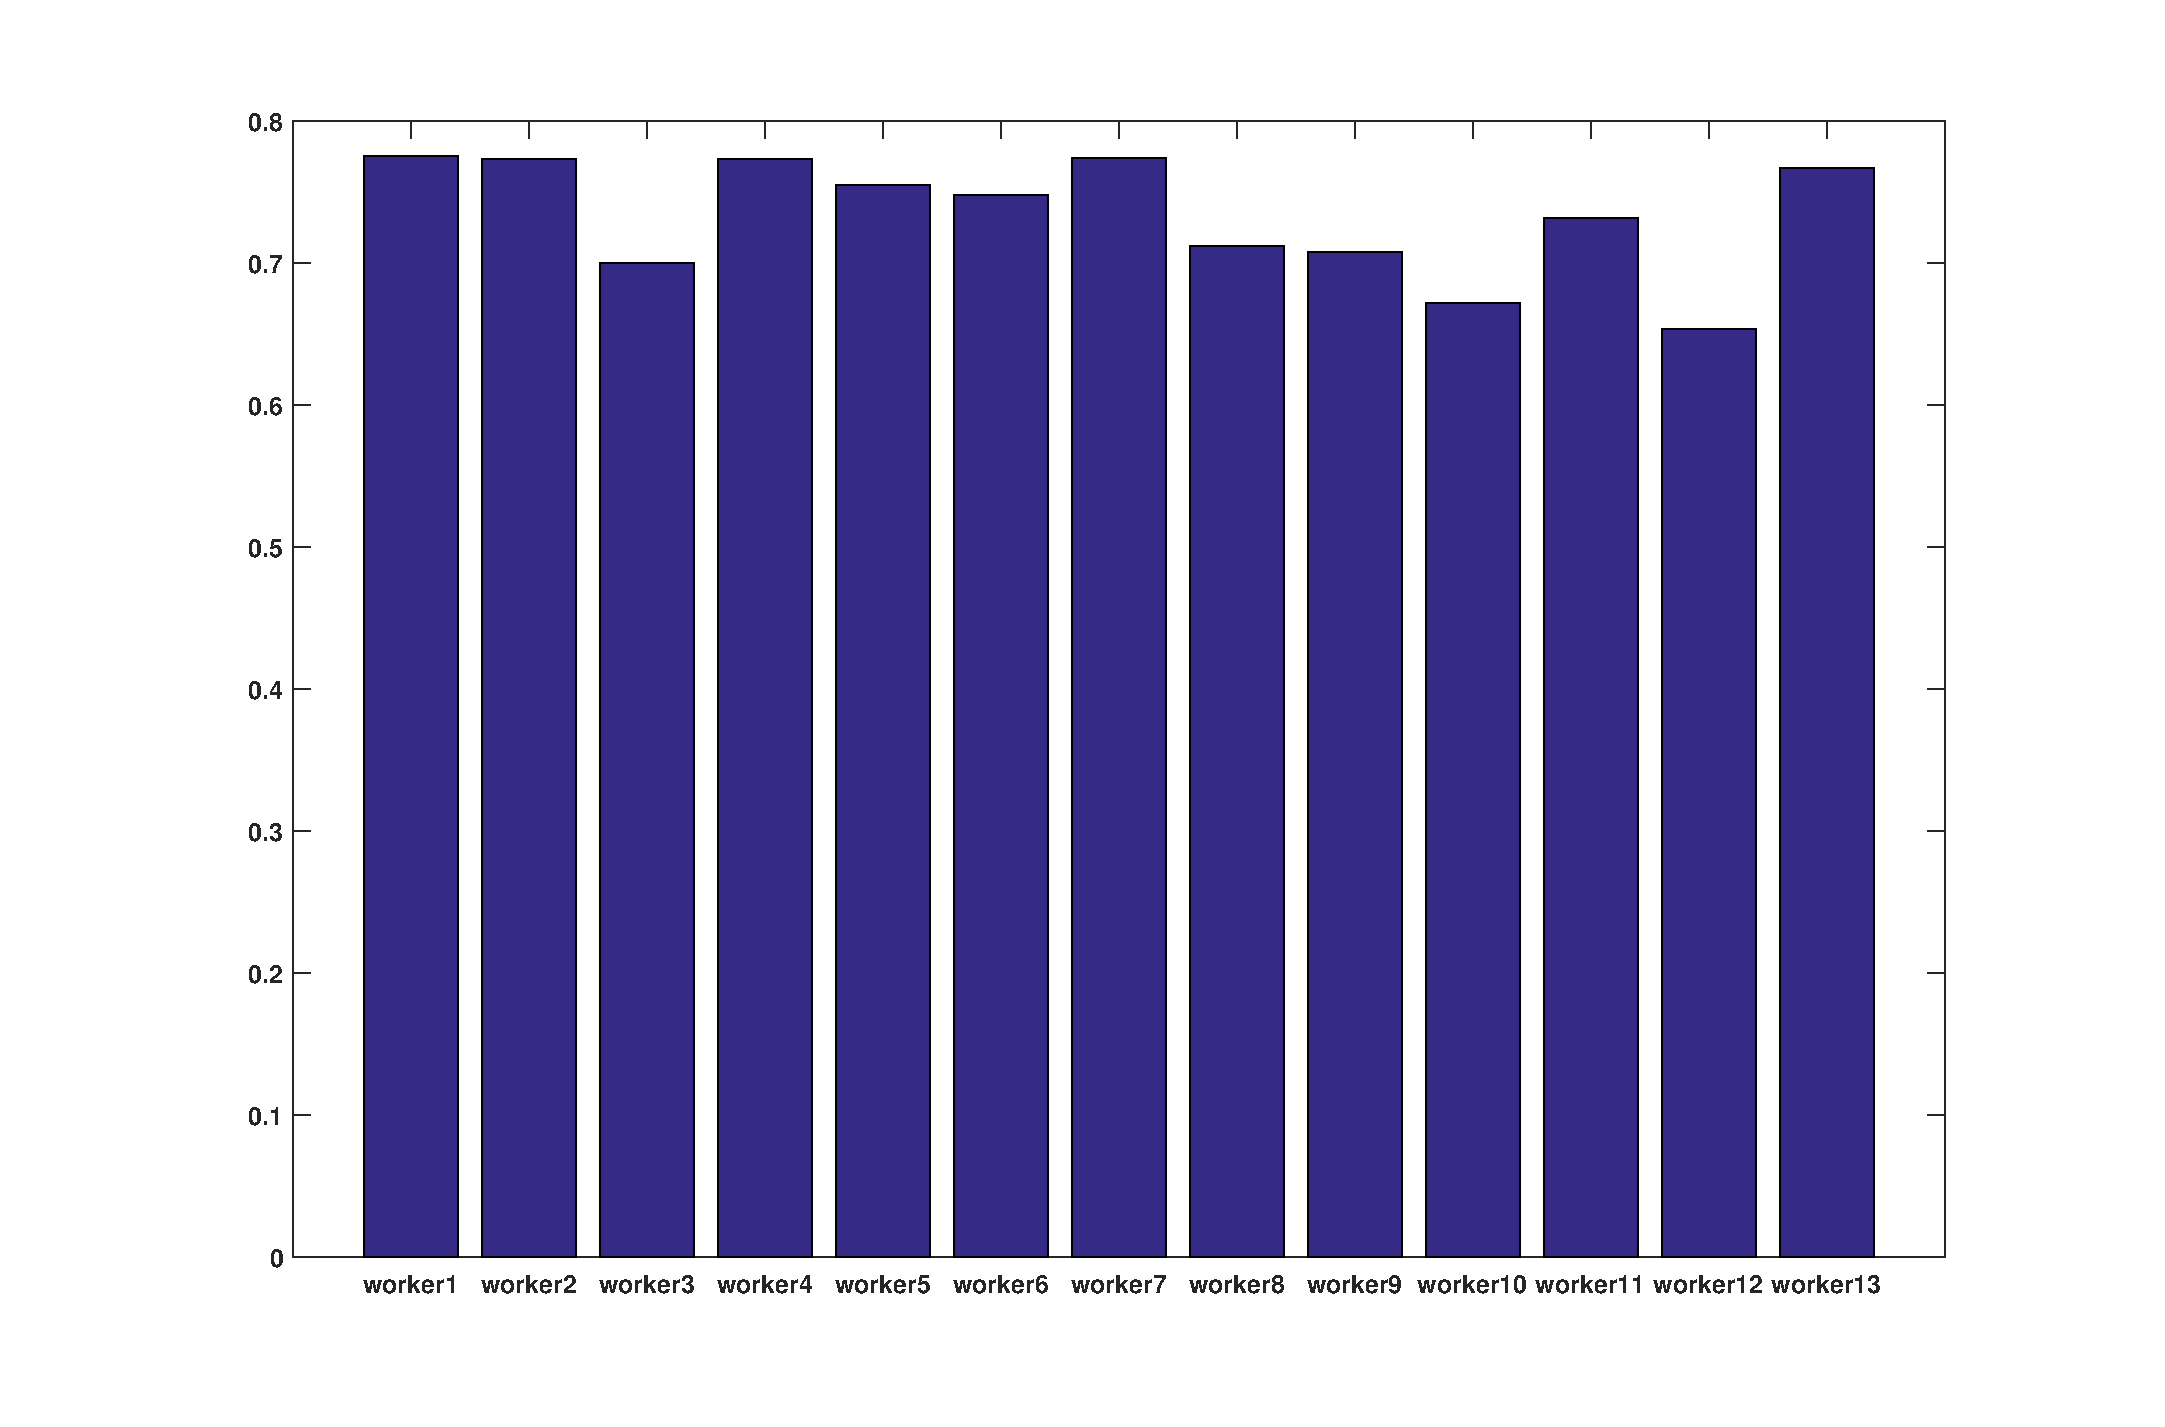
\includegraphics[width = 0.8\linewidth]{figures/mean_pairwise_correlation_without_work4.eps}
\caption{Pairwise average correlation correlation coefficients for each worker.}
\label{fig:pairwise_corr}
\end{figure}

\begin{figure}[h]
        \begin{minipage}[t]{0.5\linewidth}
        \centering
            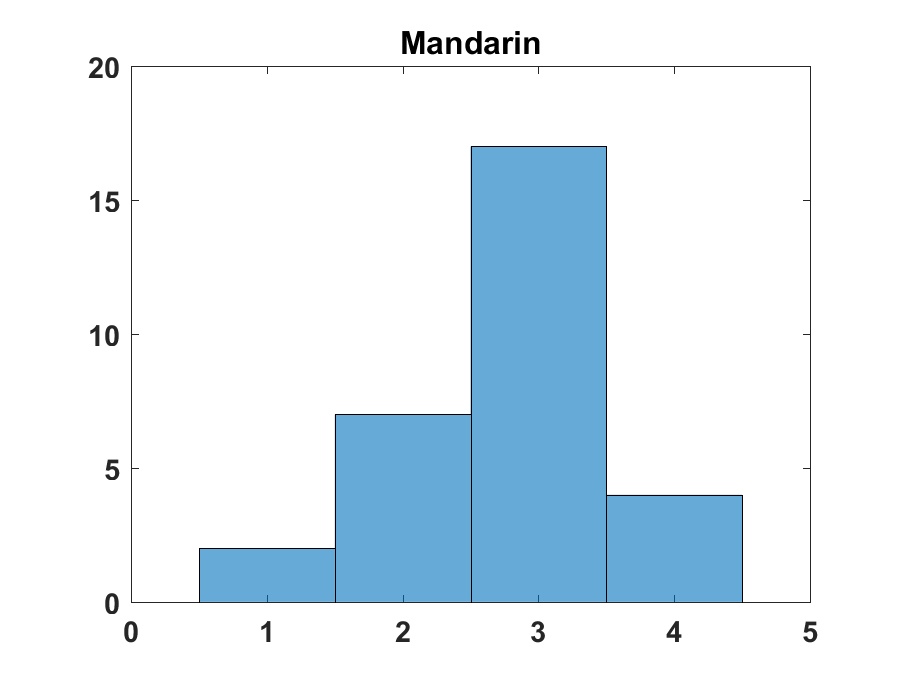
\includegraphics[width=3in]{figures/Mandarin_hist.eps}
        \end{minipage}%
        \begin{minipage}[t]{0.5\linewidth}
        \centering
            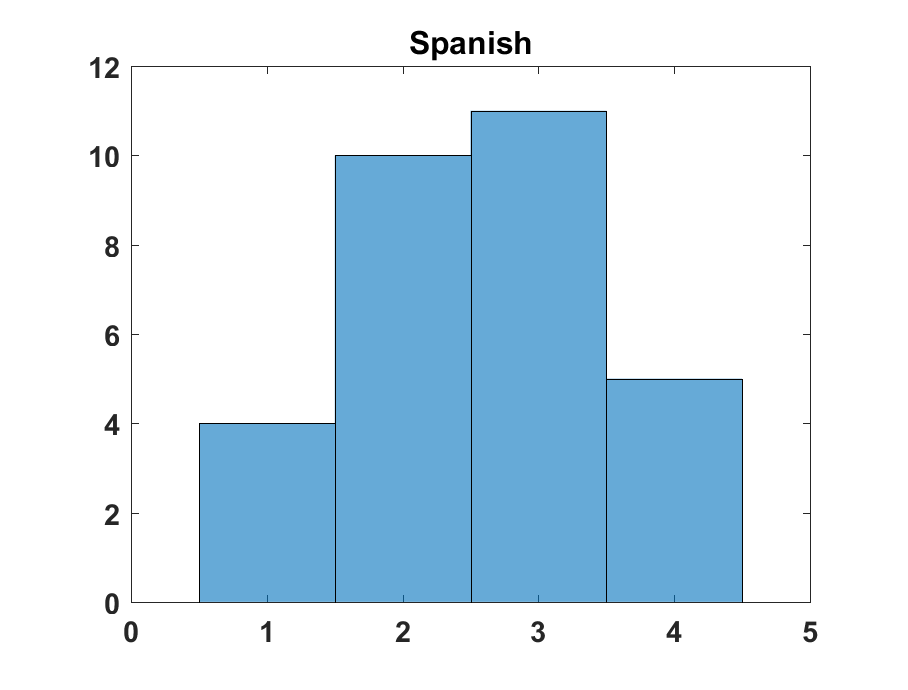
\includegraphics[width=3in]{figures/Spanish_hist.eps}
        \end{minipage}%
        \\
        \begin{minipage}[t]{0.5\linewidth}
        \centering
            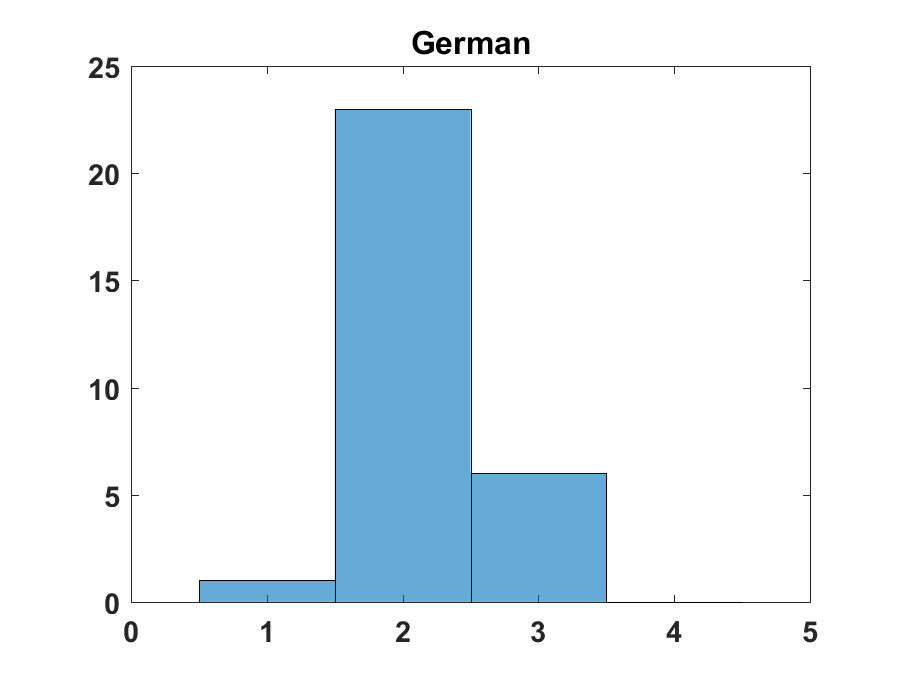
\includegraphics[width=3in]{figures/German_hist.eps}
        \end{minipage}%
        \begin{minipage}[t]{0.5\linewidth}
        \centering
            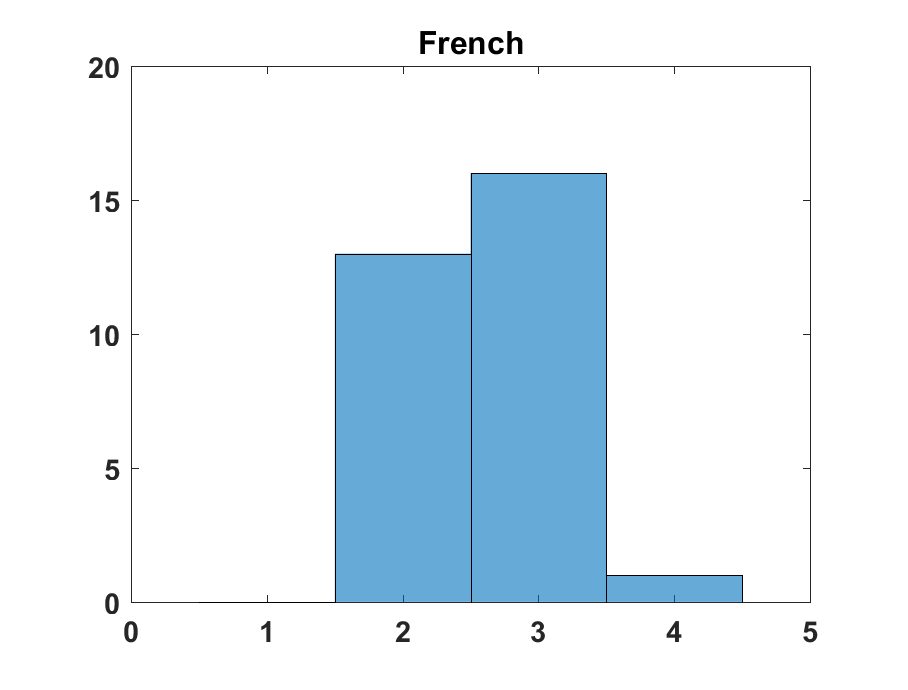
\includegraphics[width=3in]{figures/French_hist.eps}
        \end{minipage}%
        \caption{Histograms of accentedness scores of different L1s.}
        \centering
        \label{fig0}
     \end{figure}

\section{Acoustic analysis}

With the accentedness score for each speakers in the accented speech dataset collected, next step is to extract measurements from the acoustic signal to represent the foreign accent of each speaker. As mentioned in chapter \ref{introduction}, this study will analyze acoustic measurements in two subspaces: one is characterized by phonetic measurements and the other is characterized by prosodic measurements. Thus, the acoustic analysis here is also done in the two subspaces. Specifically, pronunciation scores of phonemes (including vowels and consonants) and syllables are calculated as representation of the phonetic subspace. The pronunciation scores are calculated based on previous studies on phoneme-level goodness of pronunciation \citep{witt2000phone}, which relies on a already-trained automatic speech recognition (ASR) system on native L2 speech. Prosodic measurements are calculated based on the studies by \cite{ramus1999correlates,grabe2002durational}. In this dissertation, more prosodic measurements are included compared by the previous studies as in \citep{lai2013applying}. Furthermore, the main contribution of this study is to investigate the relationship between L1 related acoustic measurements and accentedness score. To calculate L1 related acoustic measurements, corpus of different L1s (German, French, Spanish and Mandarin in this study) are also needed. The remaining part of this section will first briefly review the basic concepts of an ASR system. Then, L1 corpus used in this study will be introduced. Finally, acoustic feature extraction scheme for both phonetic and prosodic information will be presented.

\subsection{A brief introduction to ASR}

\begin{figure}[t]
\centering
\captionsetup{justification=centering}
\includegraphics[width = 1.0\linewidth]{figures/ASR_diagram.pdf}
\caption{Diagram of a typical ASR system. The content of the speech signal is ``what do you mean''.}
\label{fig:asr_diagram}
\end{figure}

 Basically, ASR is trying to recognize the content, i.e. what the speaker is saying, in a speech signal. It requires knowledge from different fields, including psychoacoustics and signal processing, linguistics and machine learning\footnote{Recent developments on ASR mainly focus on the machine learning part.}. A simplified diagram of an ASR system is shown in figure \ref{fig:asr_diagram}. The input waveform is first analyzed within short windows (e.g. 25ms), also referred as frames, based on the assumption that spectral information is stationary in a short window. This process is done frame by frame. Then, a feature (usually based on Discrete Fourier Transformation) vector is calculated to represent the spectral information in each frame. The 1-dimensional time domain signal is then converted to a 2-dimensional time-frequency representation. Since phonemes can be discriminated based on spectral information in acoustic signal, this feature vector is believed to carry information of the identity of phoneme.

 \begin{figure}[t]
\centering
\captionsetup{justification=centering}
\includegraphics[width = 0.4\linewidth]{figures/HMM_state.JPG}
\caption{How an HMM aligns input feature vectors with output state sequence.}
\label{fig:hmm_diagram}
\end{figure}

 The feature vectors of a sentence is sent to recognizer, which includes three parts: acoustic model, language model and pronunciation model. Acoustic model builds the relationship between feature representation and phonemes. A sequence machine learning model called Hidden Markov Model (HMM) is employed to learn the dynamic transition from one phoneme to another based on observed feature vectors in each short window by aligning each frame with a state of HMM model. The reason to use HMM is that the number of frames is different from the number of phonemes in a sentence. There must be a way to correspond each frame to a sub-phoneme unit, which is called a state in HMM. Each HMM models one phonemes and the final acoustic model will have many HMMs. As the HMM shown in figure \ref{fig:hmm_diagram}, input feature vectors $o_1$ to $o_6$ are mapped to a state sequence $s_1$ to $s_6$, each of which corresponds to state IDs $\{1,2,3\}$. At each frame, it either moves to the next state or stay at the current state. State 0 and 4 are the entrance and exit state of the HMM, which allows transition from a previous phoneme and exit from the current phoneme. Most of the time, a triphone([k-ae+t], [k] is to the left of [ae] and [t] is to the right) instead of a single phone([ae]) is used as the basic modeling unit of an HMM for the reason that triphone can better model the coarticulation among neighboring phonemes and improve model capability. In summarization, the acoustic model converts a sequence of feature vectors to a sequence of HMM states, and then to phoneme sequence according to the mapping between HMM states to phonemes.

 The language model is for converting phoneme sequence output by acoustic model to feasible word sequences which complies with human usage of words. The pronunciation model involves in this process: it gives the phoneme sequence of each single word in a language. In a nutshell, pronunciation model is just the lexicon(or dictionary) of a language in most of the time. Pronunciation model will also be used to convert word sequences in transcription to phoneme sequences during training of the acoustic mode. There is another term commonly seen in ASR field: forced-alignment. It refers to the process to find the start and end time of a phoneme, word or even sentence in a speech signal given the transcription. This can be achieved using acoustic model and pronunciation model. A lot of studies in computational linguistics use forced-alignment to avoid locating phonemes and words in a speech signal by hand. Practically, Kaldi toolkit \citep{povey2011kaldi} is the most commonly used software to build an ASR system and it has been well accepted by academia and industry.

\subsection{Native speech corpus}
In this study, both the L2 and L1s acoustic models are needed to extract pronunciation score based phonetic features. To build the L2 acoustic model (English for this study), the LibriSpeech corpus \citep{panayotov2015librispeech} was used and the corresponding training scripts\footnote{https://github.com/kaldi-asr/kaldi/tree/master/egs/librispeech/s5} in the Kaldi toolkit. The final acoustic model is a triphone model trained with Gaussian Mixture Model-Hidden Markov Model on 960 hours of speech data. The feature input is a 39-dimensional second order Mel-Frequency Cepstral Coefficient (MFCC) with utterance-level cepstral mean variance normalization and Linear Discriminant Analysis transformation.

For Mandarin, the publicly accessible AIShell Mandarin Speech corpus (approximately 150 hours training data) \citep{bu2017aishell} and the corresponding Kaldi scripts\footnote{https://github.com/kaldi-asr/kaldi/tree/master/egs/aishell/s5} are used. A pronunciation dictionary is included with the dataset. For the remaining three languages (Spanish, French and German), there are no well organized publicly available data. We use data from the Voxforge project and download the speech corpora for French ($\approx$ 30 hours), German ($\approx$ 50 hours) and Spanish ($\approx$ 50 hours). Kaldi scripts\footnote{https://github.com/kaldi-asr/kaldi/tree/master/egs/voxforge/s5} for the Voxforge The dictionary for these three languages are from the CMU Sphinx (Download available\footnote{https://sourceforge.net/projects/cmusphinx/files/Acoustic\%20 \\ \hspace*{4mm} and\%20Language\%20Models/}). Feature types and structures of acoustic models for the four languages are the same as those used in the English acoustic model.

\subsection{Pronunciation score based phonetic feature extraction}
\label{sec:segmental}

\subsubsection{Features based on the L2 acoustic model}
\label{sec:L2_measure}

Motivated by the work by \cite{witt2000phone}, the goodness of pronunciation for each phoneme is calculated in the accented speech. To do this, the accented speech is first force-aligned at the phoneme-level using the L2 acoustic model to provide the start and end frame indices of each phoneme. The pronunciation score ($PS_{\mathrm{L2}}$) of the target phoneme $p$ after alignment is defined as
\begin{equation}
\label{gop}
\begin{aligned}
PS_{\mathrm{L2}}(p) &= \log(P(p|\mathbf{O}^{p}))/\left | \mathbf{O}^{p} \right | \\
      &= \log \left [ \frac{P(\mathbf{O}^{p}|p)P(p)}{\sum_{q\in \mathit{Q}} P(\mathbf{O}^{q}|q)P(q)} \right ] /\left | \mathbf{O}^{p} \right |,
\end{aligned}
\end{equation}
where $\mathbf{O}^{p}$ is the feature matrix of phoneme $p$, $\left |\mathbf{O}^{p}\right |$ is the number of frames of phoneme $p$ after alignment, and $\mathit{Q}$ is the set of all phonemes. If we assume equal priors for all phonemes, we approximate the denominator in Eq. \ref{gop} with max operator,

\begin{equation}
\label{gop2}
PS_{\mathrm{L2}}(p) = \log \left [ \frac{P(\mathbf{O}^{p}|p)}{\max_{q\in \mathit{Q}} P(\mathbf{O}^{q}|q)} \right ] /\left | \mathbf{O}^{p} \right |.
\end{equation}

The conditional likelihood of each phoneme (given the speech frames of the corresponding aligned segment) can be calculated by decoding the sequence of speech features using the L2 acoustic model. It is clear that if the most likely phoneme returned by the acoustic model is the same as the target phoneme $p$, then $PS_{\mathrm{L2}}(p)=0$; otherwise, this value will be negative. The interpretation is that the closer $PS_{\mathrm{L2}}(p)$ is to zero, the closer the pronunciation of phoneme $p$ is to that of native speakers.

\subsubsection{L1 acoustic model based measurements}
\label{sec:L1_measure}

In contrast to the $PS_{\mathrm{L2}}$ score, there is no transcript to measure the pronunciation of the phonemes in L1. We define a new way to calculate the pronunciation score with the L1 acoustic model which quantifies how close the pronunciation of a phoneme in L2 is to a specific phoneme in L1. The forced-alignment calculated with the L2 acoustic model is used here. The speech frames are first decoded with the L1 acoustic model and find the state path with the highest likelihood. In the path, the corresponding phonemes of each HMM state are recorded and the phoneme with the highest occurrence is considered as the most likely L1 phoneme for a given speech segment. Then, the pronunciation score is calculated as

\begin{equation}
\label{l1gop}
PS_{\mathrm{L1}}(p) = \left [ \sum_{t \in T_p} \log \frac{ \sum_{s \in S_p}P(o_t|s)}  { \sum_{s \in S}P(o_t|s)} \right ] /\left | T_p \right |,
\end{equation}
where $o_t$ is the feature vector for frame $t$ and $p$ is the phoneme with the highest occurrences in the best decoding path of the current segment. $T_p$ is the set of frames where each frame corresponds to an HMM state of phoneme $p$. $S_p$ is the set of HMM states that belong to phoneme $p$ and $S$ is the set of all HMM states. $PS_{\mathrm{L1}}(p)$ essentially quantifies the confidence of the L1 acoustic model that phoneme $p$ was produced for a speech segment. With equation \ref{l1gop}, a pronunciation score based on the L1 acoustic model can be calculated for each phoneme segment in the original alignment. The implementations of both feature sets are available on Github\footnote{https://github.com/tbright17/kaldi-dnn-ali-gop}.

\subsubsection{Sentence-level integration}

Previous introduced feature extraction methods will output both $PS_{\mathrm{L2}}$ and $PS_{\mathrm{L1}}$ on phoneme level. However, accented speech of each speaker is a sentence. Thus, a sentence-level integration method is proposed to convert phoneme-level pronunciation scores to a sentence-level feature vector. Specifically, after phoneme-level features $PS_{\mathrm{L2}}(p)$ and $PS_{\mathrm{L1}}(p)$, are extracted, \a sentence-level feature extraction scheme was used to convert phoneme-level measurements to a feature vector with a fixed dimension for each utterance. The pronunciation features for vowels, consonants and syllables are first grouped together and four statistics for each of these three phonetic categories are then calculated: for both $PS_{\mathrm{L2}}(p)$ and $PS_{\mathrm{L1}}(p)$, the minimum, mean, standard deviation and mean-normalized standard deviation (standard deviation divided by mean) of phoneme-level pronunciation measurements of vowels, consonants and syllables in each utterance are calculated (implementation available\footnote{https://github.com/tbright17/accent-feat}). This results in a total of 12 utterance-level features for the acoustic model of each language, and a total of 24 utterance-level features combining both pronunciation information from L1 and L2 acoustic models.

\subsection{Prosodic feature extraction}
\label{sec:supraseg}

To represent speech prosody, durational rhythmic measurements of phonemes and syllables are adopted as the studies by \cite{ramus1999correlates,grabe2002durational}. Specifically, an extended speech rhythmic feature set proposed in \citep{lai2013applying} are employed in this study. First, the same forced-alignment results achieved in previous section is reused here to get the start and end time of each phoneme. Then, the following measurements are calculated:
\begin{enumerate}
\item Mean, standard deviation and mean-normalizd standard deviation (standard deviation divided by mean) of durations of vowels, consonants and syllables.
\item Duration proportion of vowels, consonants and syllables, calculated as the total length of vowels, consonants and syllables divided by the length of the sentence.
\item Raw Pairwise Variability Index (rPVI) of durations of vowels, consonants and syllables, calculated as:
    \begin{equation}
    \label{eq:rPIV}
    rPVI= \sum_{k=1}^{m-1} |d_k-d_{k+1}|/(m-1),
    \end{equation}
    where $d_k$ is the duration of $k$th phoneme or syllable and $m$ is the total number of phonemes or syllables in a sentence.
\item Normalized Pairwise Variability Index (nPVI) of durations of vowels, consonants and syllables, calculated as:
    \begin{equation}
    \label{eq:nPIV}
    nPVI= \sum_{k=1}^{m-1} |\frac{d_k-d_{k+1}}{(d_k + d_{k+1})/2}|/(m-1),
    \end{equation}
    where the notations are the same as in equation \ref{eq:rPIV}.
\end{enumerate}

Finally, a 18-dimensional feature vector can be extracted from each speech signal. In this study, this rhythmic feature extraction scheme is applied to both L1 speech, L2 speech and accented speech to do contrastive analysis between accented speech and L1 and between L2 speech and accented speech. For the four foreign languages, 1000 sentences with more than 40 phonemes are randomly selected from the corresponding native speech corpus. For native English, those measurements are directly calculated on the 30 native American English sentences from SAA.

\section{Procedure}

 \begin{figure}[t]
\centering
\captionsetup{justification=centering}
\includegraphics[width = 0.8\linewidth]{figures/method_diagram.pdf}
\caption{Diagram of the methodology used in this study.}
\label{fig:method_diagram}
\end{figure}

The diagram of the methodology used in this study is shown in figure \ref{fig:method_diagram}. After extracting acoustic measurements from native L1 speech, accented speech and native L2 speech, contrastive analysis, the goal of which is to quantify the difference between two sets of features is applied on the L1-accented pair and L2-accented pair. Then two sets of features can be obtained: the L2 normalized acoustic measurements represent how close the phonological properties in accented speech is to native L2 speech; the L1 normalized acoustic measurements represent how close the phonological properties in accented speech is to native L1 speech. The segmental feature extraction scheme in section \ref{sec:segmental} directly output the L1 and L2 normalized acoustic measurements because the input of the method is accented speech and L1 or L2 acoustic model and the output is already contrastive. In contrast, contrastive analysis needs to be done for the supra-segmental feature extraction method in section \ref{sec:supraseg}. Both these two sets of features can be further categorized into segmental measurements and supra-segmental measurements. The first data analysis, which will be introduced in chapter \ref{l1_seg}, will investigate the effect of L1 phonological properties on the phonetic system of accented speech.  The second data analysis, which will be introduced in chapter \ref{l1_supraseg}, will investigate the effect of L1 phonological properties on the prosodic system of accented speech. The third data analysis, which will be introduced in chapter \ref{both_l1_l2}, will investigate the effect of L1 phonological properties on both the phonetic and prosodic systems of accented speech and propose a new computational model to do automatic accentedness evaluation. The data analysis methods used in this study are mainly the correlational analysis, which examines how the acoustic measurements and accentedness score are correlated, and multiple regression analysis, which examines how well the combination of multiple acoustic measurements can predict the accentedness score. The data analysis procedure involves feature preprocessing, feature selection and mode regularization, which will be introduced in detail in later chapters. 
\chapter{L1's effect on phonetic properties of accented speech}
\label{l1_seg}

\section{Introduction}

This section will investigate the statistical relationship between the phonetic acoustic measurements extracted from accented American English speech (independent variables) and the perceived accetendenss score provided by native American English speakers (dependent variables). Two sets of features will be used as independent variables: one is the pronunciation score based features extracted only using L2 acoustic model and the other one is the pronunciation score based features extracted using both L1 and L2 acoustic model. This corresponds to the data analysis 1 in figure \ref{fig:method_diagram} using only L2 normalized segmental acoustic measurements and the combination of  both L1 and L2 normalized segmental acoustic measurements. First, correlational relationship between independent variables and dependent variables. Second, multiple regression analysis will be employed to analyze how well each set of features can predict the accentedness score. Results and discussion are in the final part.

\section{Methods}


For each foreign language, the correlation analysis will be done between each dimension of the feature vector and the accentedness scores ( average of all 13 annotators). 
\chapter{L1's effect on prosodic properties of accented speech}
\label{l1_supraseg}

\section{Introduction}

The previous chapter applies the proposed methodology for accentedness perception to pronunciation based segmental features and proves that integrating L1 pronunciation information by extracting pronunciation score of accented English speech with L1 acoustic model can improve the prediction accuracy of accentedness perception. This chapter will focus on apply the same methodology to speech prosodic features to study whether L1 prosodic patterns affect the perception of accentedness. As mentioned in chapter \ref{sec:methodology}, durational rhythmic features will be used as proxy of speech prosody. The methods and analysis of results are almost the same as chapter \ref{l1_seg}. Details will be introduced in following sections.

\section{Methods}

In chapter \ref{sec:methodology}, the procedure to extract durational rhythmic features is introduced. The extracted rhythmic features for native L1, accented L2 speech and native L2 are represented with $\mathbf{x_{L1}}$, $\mathbf{X_{acc}}$ and $\mathbf{x_{L2}}$ respectively. Note that $\mathbf{x_{L1}}$ and $\mathbf{x_{L2}}$ are vectors because they are the average of features extracted from multiple speech recordings. These three sets of features are converted to accent related features by taking the absolute difference between $\mathbf{x_{L1}}$ and $\mathbf{X_{acc}}$ and $\mathbf{x_{L2}}$ and $\mathbf{X_{acc}}$. $\left| \mathbf{x_{L2}}-\mathbf{X_{acc}} \right|$ represent the difference between the rhythmic patterns of accented speech and target L2 speech while $\left| \mathbf{x_{L1}}- \mathbf{X_{acc}} \right|$ represents the difference between the rhythmic patterns of accented speech and speaker's L1 speech. Here, the subtraction is broadcasted to every row of $\mathbf{X_{acc}}$ to get the contrastive information for each speaker with accent.

The first analysis is the correlation analysis between speech prosodic features and accentedness score averaged of 13 annotators. Similarity, the PCC is calculated between every features of the 18-dimensional feature vectors in a language-dependent way. The procedure is different from previous chapter observing that the feature dimension is higher than pronunciation features, here only the top-12 features with highest PCC with accentedness scores are shown for each language together with the p-values (lower p-value stands for more statistically significant correlation).

Same multiple regression analysis is done here except that the number of input features is changed to 18. Downsampling is not used here since it does not help for German speakers. Thus, for each language, multiple regression analysis is done between 18-dimensional speech rhythmic measurements and accentedness  scores of 30 speakers. Specifically, $\left| \mathbf{x_{L2}}-\mathbf{X_{acc}} \right|$ is used as the baseline model which on takes the difference of speech rhythmic patterns between accented speech and L2 into consideration. Then, $\left| \mathbf{x_{L1}}- \mathbf{X_{acc}} \right|$ can be combined into the baseline feature set to model the distance between accented speech and L1 on suprasegmental feature space. Finally, input to the baseline model is a 18-dimensional feature vector while input to the proposed model is a 36-dimensional feature vector.

As in chapter \ref{l1_seg}, the input feature vectors are first normalized with mean and standard deviation on each dimension. Then, a feature selector based on univariate regression test is applied to select the most predictable features. Ridge regression is used to learn the relationship between input features and accentedness score. The same leave-one-speaker-out CV is employed to evaluate the performance on accentedness prediction. Hyperparameters including number of features selected and strength of 2-norm regularization in ridge regression are tuned to achieve the best CV performance. PCC and MAE are reported language dependently. To better illustrate the process, figure \ref{fig:l1_supraseg_diagram} shows the whole procedure of multiple regression analysis.

\begin{figure}[t]
        \begin{minipage}[t]{1.0\linewidth}
        \centering
            \includegraphics[width=5.0in]{figures/method_diagram_supraseg.pdf}
        \end{minipage}%
        \caption{Diagram of the procedure for multiple regression analysis between suprasegmental prosodic features and accentedness scores. Here, $\mathbf{x_{L1}}$ and $\mathbf{x_{L2}}$ are the average of features of all speech recordings. $\mathbf{x_{acc}}$ is the feature vector for one accented speech recording.}
        \centering
        \label{fig:l1_supraseg_diagram}
     \end{figure}

\section{Results}
\subsection{Results of correlation analysis}

\begin{figure}[]
        \begin{minipage}[t]{0.5\linewidth}
        \centering
            \includegraphics[width=3in]{figures/supra_seg_bar_plot/german.pdf}
        \end{minipage}%
        \begin{minipage}[t]{0.5\linewidth}
        \centering
            \includegraphics[width=3in]{figures/supra_seg_bar_plot/french.pdf}
        \end{minipage}%
        \\
        \begin{minipage}[t]{0.5\linewidth}
        \centering
            \includegraphics[width=3in]{figures/supra_seg_bar_plot/mandarin.pdf}
        \end{minipage}%
        \begin{minipage}[t]{0.5\linewidth}
        \centering
            \includegraphics[width=3in]{figures/supra_seg_bar_plot/spanish.pdf}
        \end{minipage}%
        \caption{Bar plots of the top-12 features highly correlated with accentedness scores in feature sets $\left| \mathbf{x_{L2}}-\mathbf{X_{acc}} \right|$ (upper panel in each subfigure) and $\left| \mathbf{x_{L1}}- \mathbf{X_{acc}} \right|$ (lower panel in each subfigure). Y-axis is the correlation coefficients with accentedness score and X-axis is feature names. The numbers on top of each bar are the p-value for testing non-correlation.}
        \centering
        \label{fig:supraseg_bar}
     \end{figure}

In figure \ref{fig:supraseg_bar}, PCC together with p-value between two sets of speech rhythmic features and accentedness scores of four different foreign languages are presented. Feature names on X-axis are abbreviations: per\{V,C,Syl\} represents the percentage of durations of vowels, consonants and syllables, avg\{V,C,Syl\} represents the average durations, std\{V,C,Syl\} represents the standard deviation of durations, Vacro\{V,C,Syl\} represents the mean-normalizd standard deviation of durations, rPVI\{V,C,Syl\} represents the Raw PVI of durations and nPVI\{V,C,Syl\} represents the Normalized PVI) of durations. From the figure, there are several interesting observations:

\begin{enumerate}
\item Except for German speakers, other three languages all have relatively high correlation coefficients ($>$0.6) with accentedness scores. This can be attributed to the similarity of rhythmic patterns between English and German (as shown in figure \ref{fig:rhythmic_mds} and table \ref{table:conf_rhythmic}, also in the study by \cite{li2014l2}). It becomes hard to use rhythmic features to differentiate between mild and strong accent when the rhythmic patterns of L1 is already very close to L2.
\item As shown in previous chapter, the most predictable features extracted with L1 acoustic models have opposite correlation with accentedness scores compared to features extracted with L2 acoustic models. However, for rhythmic features, it can be found that most features of both $\left| \mathbf{x_{L2}}-\mathbf{X_{acc}} \right|$ and $\left| \mathbf{x_{L1}}- \mathbf{X_{acc}} \right|$ are positively correlated with accentedness scores. Only a few dimensions of $\left| \mathbf{x_{L1}}- \mathbf{X_{acc}} \right|$ have negative correlation with accentedness scores. This indicates that for some speakers, values of feature dimensions in $\mathbf{X_{acc}}$ are not within the range from values of $\mathbf{x_{L2}}$ to values of $\mathbf{x_{L2}}$ in corresponding dimensions while values on some feature dimensions are between the values in L1 and L2. This is also observed in the study by \cite{white2007calibrating}. This observation is consistent with the founds in \citep{li2014l2} where the authors believe that for speech rhythm acquisition there is a multisystemic model of L2 rhythm acquisition and both transferred L1 knowledge and universal effects independent of L1 played a role.
\item For languages that have high correlation coefficients, it can be found that the average durations features and PVI features are the most correlated ones. This is also consistent with studies by \cite{ordin2015acquisition} where they show the different rhythmic feature values in different proficiency levels: beginners, intermediate and advanced although they did not provide correlation coefficients between rhythmic feature values and how strong the accent is.
\end{enumerate}

\subsection{Results of multiple regression analysis}

During the experiment, it was found that For French and Mandarin, using feature set [$\left| \mathbf{x_{L2}}-\mathbf{X_{acc}} \right|$, $\left| \mathbf{x_{L2}}-\mathbf{X_{acc}} \right|$-$\left| \mathbf{x_{L1}}- \mathbf{X_{acc}} \right|$] as the way to integrate L1 information gave the best performance of leave-one-speaker-out CV; for Spanish speaker, feature set [$\left| \mathbf{x_{L2}}-\mathbf{X_{acc}} \right|$, $\left| \mathbf{x_{L1}}- \mathbf{X_{acc}} \right|$] gave the best performance. Since for French and Mandarin, using [$\left| \mathbf{x_{L2}}-\mathbf{X_{acc}} \right|$, $\left| \mathbf{x_{L1}}- \mathbf{X_{acc}} \right|$] can also achieve better performance than the baseline model, the difference of the best feature sets across languages is probably due to different speech prosody patterns.
In table \ref{table:supraseg_pred}, both the PCCs and MAEs between model predicted accentedness and human annotated accentedness for 3 groups of speakers are presented. Here, the results for German speakers are not showed because the prediction of the regression model is pretty bad and has negative correlation with human accentedness scores. Downsampling did not help in this case. This is consistent with the correlation analysis in figure \ref{fig:supraseg_bar}, where German rhythmic features have low correlation with accentedness score. There is no downsampling for French seapekrs either because without downsampling, the performance on French speakers is already satisfied. There is a consistent improvement when adding L1 rhythmic patterns based features for all 3 L1s. These results show that there is an improvement in model performance consistently and across all three languages after adding features from contrastive information with L1 rhythmic patterns. It proves that the rhythmic contrastive information between accented speech and L1 can provide extra information for accentedness prediction. This is also despite the fact that the annotators know little about the acoustic properties of the speakers' L1s.

\begin{table}[]
\centering
\caption{PCCs and MAEs between predicted accentedness and human scores for speakers of three different L1s.}
\label{table:supraseg_pred}
\begin{tabular}{|c|c|c|c|c|}
\hline
 & \multicolumn{2}{c|}{[$\left| \mathbf{x_{L2}}-\mathbf{X_{acc}} \right|$]} & \multicolumn{2}{c|}{With $\left| \mathbf{x_{L1}}- \mathbf{X_{acc}} \right|$} \\ \hline
 & PCC & MAE & PCC & MAE \\ \hline
French & 0.647 & 0.310 & 0.680 & 0.289 \\ \hline
Mandarin & 0.581 & 0.425 & 0.712 & 0.380 \\ \hline
Spanish & 0.698 & 0.507 & 0.729 & 0.482 \\ \hline
\end{tabular}
\end{table}

\begin{table}[]
\centering
\caption{Selected feature dimensions from [$\left| \mathbf{x_{L2}}-\mathbf{X_{acc}} \right|$, $\left| \mathbf{x_{L2}}-\mathbf{X_{acc}} \right|$-$\left| \mathbf{x_{L1}}- \mathbf{X_{acc}} \right|$] for French and Mandarin speakers or [$\left| \mathbf{x_{L2}}-\mathbf{X_{acc}} \right|$, $\left| \mathbf{x_{L1}}- \mathbf{X_{acc}} \right|$] for Spanish speakers. ``num\_feature'' stands for the total number of selected features by feature selection.}
\label{table:supraseg_feat_sel}
\begin{tabular}{|c|c|l|l|l|}
\hline
 & \multicolumn{4}{c|}{Selected feature dimensions} \\ \hline
\begin{tabular}[c]{@{}c@{}}French \\ (num\_feat=25)\end{tabular} & \multicolumn{4}{c|}{\begin{tabular}[c]{@{}c@{}}avgC, avgSyl, stdC, stdSyl,VacroC, \\ perC, perSyl, rPVIC, rPVISyl, nPVISyl\end{tabular}} \\ \hline
\begin{tabular}[c]{@{}c@{}}Mandarin \\ (num\_feat=15)\end{tabular} & \multicolumn{4}{c|}{avgV, avgC, stdV,perV} \\ \hline
\begin{tabular}[c]{@{}c@{}}Spanish \\ (num\_feat=11)\end{tabular} & \multicolumn{4}{c|}{avgC, avgSyl, stdC, rPVIC, rPVISyl,nPVIC} \\ \hline
\end{tabular}
\end{table}

In order to show that features extracted with L1 rhythmic patterns really helps with predicting accentedness scores, in table \ref{table:supraseg_feat_sel}, L1 rhythmic patterns based features that are selected to predict accentedness scores are showed. Since the multiple regression analyses are done language-independently, different sets of features are selected for different languages, and the number of features selected for each language is also presented in the table. It can be found that for French and Spanish speakers, the durational measurements of L1 consonants and syllables are more import features while for Mandarin speakers the durational measurements of L1 vowels are more import features. The study by \cite{li2014l2} compared durational measurements of Mandarin accented English and native English. They showed that vocalic rhythmic measurements can well discriminate Mandarin learners at different proficiency levels. While for French and Spanish speakers, there are no studies showing the progressive change of consonantal and syllable rhythmic measurements along the proficiency level. The results here are reasonable considering both French and Spanish are syllable-timed languages while English is stress-timed languages. The results of the multiple regression analysis further validate the hypothesis in chapter \ref{introduction} that ``If this distance information is added to the feature sets for automatic accentedness evaluation, the performance will be improved.

\section{Discussion}

This chapter shows that the speech prosodic properties transferred from L1 can also help deciding how strong the foreign accent is for L2 learners. This conforms with previous studies where they show the L1 effect in L2 prosody acquisition \citep{rasier2007prosodic,stockmal2005measures,white2007calibrating,li2014l2,ordin2015acquisition}. However, based on the correlation analysis in figure \ref{fig:supraseg_bar}, on most feature dimensions, it does not indicate that if the rhythmic property on that dimension is further from L1, the foreign accent is milder. This is in contrast to the results in table \ref{table:seg_corr}. The first possible reason is that while previous studies show the effect of L1 on L2 rhythmic pattern acquisition, there are also obvious universal effect that are independent of L1. For example, the study \cite{ordin2015acquisition} showed that the PVI measurements of English speech produced by French speakers can be even higher than native English speakers given that English speech has much higher PVI measurements than French speech. The second possible reason is that all the rhythmic measurements in this study are based on automatic forced alignment. For speakers with not very strong accent, the will be much less forced-alignment errors. However, for speakers with very strong accent, the forced-alignment results may not be that accurate. This will also affect the correlation analysis between features and accentedness scores. Another interesting observation is that for German speakers, rhythmic features do not help in predicting accentedness score. This is due to the similarity between English and German rhythmic patterns. Both perceptually and computationally, it is hard to find useful rhythmic features extracted from acoustic signal that can discriminate different degrees of foreign accent.

Compared to the results in chapter \ref{l1_seg}, for German and Mandarin speakers, using only segmental pronunciation based features can better predict accentedness scores than using only supra-segmental rhythmic features; while for French and Spanish, the supra-segmental rhythmic features perform better. Compared to previous studies using phonological properties transplantation to investigate the relative importance of segmental and supra-segmental in accentedness perception, this study provide a new way to look at the same problem with the advantage that this method can provide quantitative analysis.
 
\chapter{Computational model for accentedness perception with L1 information}
\label{both_l1_l2}
\chapter{General discussion}
\label{discussion}
\include{chapter8}
%-----------------------back matter
{\singlespace
% Making the references a "part" rather than a chapter gets it indented at
% level -1 according to the chart: top of page 4 of the document at
% ftp://tug.ctan.org/pub/tex-archive/macros/latex/contrib/tocloft/tocloft.pdf
\addcontentsline{toc}{part}{REFERENCES}
\bibliographystyle{asudis}
\bibliography{dis}}
\renewcommand{\chaptername}{APPENDIX}
\addtocontents{toc}{APPENDIX \par}
\appendix
\include{appendix1}
\chapter{Consent form for accentedness score collection on AMT}
\label{sec:appendix2}



\subsubsection{Introduction}
The purposes of this form are to provide you (as a prospective research study participant) information that may affect your decision as to whether or not to participate in this research and to record the consent of those who agree to be involved in the study.
\subsubsection{Researchers}

Dr. Julie Liss, a Professor in the Department of Speech \& Hearing Sciences (College of Health Solutions) at ASU, and Dr. Visar Berisha, an Assistant Professor in the Department of Speech \& Hearing Sciences and the School of Electrical, Computer, and Energy Engineering at ASU, have invited your participation in a research study.
\subsubsection{Study purpose}
We are collecting perceived degree of accentedness from people aged 18 and older who have normal hearing. We will use these accentedness ratings to study the impact of non-native English speaker��s native language on the perceived accentedness.

\subsubsection{Description of research study}
If you decide to participate, then you will join a study involving research of the perception of accented speech. Your participation will be completely online and will last no longer than 1 hour. If you agree to participate, we ask that you be seated in a quiet room in front of a computer. You will listen to a paragraph spoken by different individuals in English and asked to give a general impression of the accentedness of each speaker on a 1-4 scale. Research completed based on these accentedness ratings will provide an understanding of the impact of non-native English speaker��s native language on perceived accentedness.

\subsubsection{Risks}
There are no known risks from taking part in this study.


\subsubsection{Benefits}
Although there may be no direct benefits to you, these transcriptions may improve our understanding of accented speech. This may, in turn, allow for the development of computer-aided second language learning system.

\subsubsection{Confidentiality}
All information obtained in this study is strictly confidential. The results of this research study may be used in reports, presentations, and publications, but the researchers will not identify you.

\subsubsection{Withdraw privilege}
Your participation in this project is completely voluntary. There is no penalty for not participating, or for choosing to withdraw from participation at any time. Your decision will in no way affect your relationship with ASU or your grade in any course.
Should you choose to withdraw from the study, your digital audio-video files will not be saved and will be discarded electronically.

\subsubsection{Costs and payments}
The researchers want your decision about participating in the study to be absolutely voluntary. Yet they recognize that your participation may pose some inconvenience. You will receive \$1.5 for your participation, paid via Amazon Mechanical Turk.

\subsubsection{Voluntary consent}
Any questions you have concerning the research study or your participation in the study, before or after your consent, will be answered by Dr. Julie Liss at (480) 965-9136.
If you have questions about your rights as a subject/participant in this research, or if you feel you have been placed at risk; you can contact the Chair of the Human Subjects Institutional Review Board, through the ASU Office of Research Integrity and Assurance, at 480-965 6788.
This form explains the nature, demands, benefits and any risk of the project. By signing this form you agree knowingly to assume any risks involved. Remember, your participation is voluntary. You may choose not to participate or to withdraw your consent and discontinue participation at any time without penalty or loss of benefit. In signing this consent form, you are not waiving any legal claims, rights, or remedies. A copy of this consent form will be offered to you.



By clicking ``Agree'', you consent to participate in the above study and indicated that:
\begin{enumerate}
\item you have read the above information
\item you voluntarily agree to participate
\item you are at least 18 years of age
\end{enumerate}

\include{vita}
\end{document}
